\section{Ecuaciones lineales de orden superior}
Las ecuaciones lineales de orden superior son de la forma $$y^{n)}(x) + a_{n-1}(x)y^{n-1)}(x) + \hdots + a_1(x)y^\prime(x)+a_0(x)y(x) = b(x)$$

Si $b(x) = 0$ entonces estamos ante una ecuación homogénea.

\vspace{5mm}
\obs
Una ecuación lineal de orden $n$ da origen a un sistema lineal de orden 1.
Supongamos que tenemos la ecuación $$y^{n)}(x) + a_{n-1}(x)y^{n-1)}(x) + \hdots + a_1(x)y^\prime(x)+a_0(x)y(x) = b(x)$$
Si denotamos
$$\begin{array}{c|c}
y = z_1 & z^\prime_1 = z_2\\
y^\prime = z_2 & z^\prime_2 = z_3 \\
\vdots & \vdots\\
y^{n-1)} = z_n & z^\prime_{n-1} = z_n
\end{array}$$
con
$$z^\prime_n = -a_0z_1-a_1z_2-\hdots-a_{n-1}z_n+b(x)$$
tenemos entonces el sistema
$$z^\prime = \begin{pmatrix}
0& 1& 0& 0& \hdots& 0\\
0& 0& 1& 0& \hdots& 0\\
0& 0& 0& 1& \hdots& 0\\
\vdots& \vdots& \vdots& \vdots& \ddots& \vdots\\
0& 0& 0& 0& \hdots& 1\\
-a_0& -a_1& -a_2& -a_3& \hdots& -a_{n-1}
\end{pmatrix}z + \begin{pmatrix}
0\\\vdots\\\vdots\\\vdots\\0\\b
\end{pmatrix}$$
Por tanto, los problemas de este tipo vendrán dados por una ecuación y $n$ datos iniciales, de forma que los datos son de la forma:
\begin{equation}
\left\lbrace
	\begin{array}{l l}
	y(x_0)\\y^\prime(x_0)\\\vdots\\y^{n-1)}(x_0)
	\end{array}
\right.
\end{equation}

Veamos el primer teorema de existencia y unicidad para este tipo de ecuaciones.
\begin{theorem}
Si $a_j(x), b(x)$ son funciones continuas en $(a,b)$ tal que $x_0 \in (a,b)$,  entonces dado un problema con datos iniciales en $x_0$ tenemos existencia y unicidad de la solución definida en $(a,b)$
\end{theorem}

\subsection{Ecuaciones homogéneas de orden superior}

Vamos a definir la estructura del conjunto de soluciones de una ecuación homogénea de orden superior

\begin{itemize}
\item Si $y_1,y_2$ son solución, $\forall \lambda\in \R$ tenemos que
\begin{equation}
\left\lbrace
	\begin{array}{l l}
		y_1+y_2 &\text{ es solución}\\
		\lambda y_1 &\text{ es solución}\\
	\end{array}
\right.
\end{equation}
\end{itemize}
Si definimos
$y_j(x)$ como solución al problema con dato

\begin{equation}
\begin{pmatrix}
y(x_0)\\y^\prime(x_0)\\\vdots\\y^{n-1)}(x_0)
\end{pmatrix} = \vec{e}_j = \begin{pmatrix}
0\\\vdots\\1\\\vdots\\0
\end{pmatrix}\longleftarrow \text{posición }j
\end{equation}
como en el caso de los sistemas lineales, tenemos que por el principio de superposición, el conjunto $$\{ y_1(x), y_2(x), \hdots, y_n(x) \}$$ es un conjunto generador de las soluciones del problema.

Para demostrar que es una base, basta con tomar el Wronskiano:

$$W(y_1, \hdots, y_n) = det\begin{pmatrix}
y_1(x)& \hdots& \hdots& y_n(x)\\
y^\prime_1(x)& \hdots& \hdots& y^\prime_n(x)\\
\vdots& & & \vdots\\
y^{n-1)}_1(x)& \hdots& \hdots& y^{n-1)}_n(x)\\
\end{pmatrix}$$

\begin{theorem}[de monotonía del Wronskiano]
Sean $y_1, \hdots, y_n$ soluciones de la ecuación homogénea. Entonces exisen dos posibilidades
\begin{itemize}
\item $W(y_1, \hdots, y_n) = 0 \ \forall x\in (a,b)$
\item $W(y_1, \hdots, y_n) \neq 0 \ \forall x\in (a,b)$
\end{itemize}
\end{theorem}
La demostración se realizará para $n=3$, aunque es equivalente para cualquier $n$.
\begin{proof}
Sabemos que el Wronskiano de $y_1, y_2, y_3$ en $x_0$ es
$$W(y_1, y_2, y_3) = \begin{vmatrix}
y_1& y_2& y_3\\
y_1^{\prime}& y_2^{\prime}& y_3^{\prime}\\
y_1^{\prime\prime}& y_2^{\prime\prime}& y_3^{\prime\prime}\\
\end{vmatrix}$$

Por tanto
$$W^\prime(y_1,y_2,y_3) = \begin{vmatrix}
y_1^\prime& y_2^\prime& y_3^\prime\\
y_1^{\prime}& y_2^{\prime}& y_3^{\prime}\\
y_1^{\prime\prime}& y_2^{\prime\prime}& y_3^{\prime\prime}\\
\end{vmatrix} + \begin{vmatrix}
y_1& y_2& y_3\\
y_1^{\prime\prime}& y_2^{\prime\prime}& y_3^{\prime\prime}\\
y_1^{\prime\prime}& y_2^{\prime\prime}& y_3^{\prime\prime}\\
\end{vmatrix} + \begin{vmatrix}
y_1& y_2& y_3\\
y_1^{\prime}& y_2^{\prime}& y_3^{\prime}\\
y_1^{\prime\prime\prime}& y_2^{\prime\prime\prime}& y_3^{\prime\prime\prime}\\
\end{vmatrix} = \begin{vmatrix}
y_1& y_2& y_3\\
y_1^{\prime}& y_2^{\prime}& y_3^{\prime}\\
y_1^{\prime\prime\prime}& y_2^{\prime\prime\prime}& y_3^{\prime\prime\prime}\\
\end{vmatrix}$$

$$W^\prime = \begin{vmatrix}
y_1& y_2& y_3\\
y_1^\prime& y_2^\prime& y_3^\prime\\
-ay^{\prime\prime}_1-by^\prime_1-cy_1&
-ay^{\prime\prime}_2-by^\prime_2-cy_2&
-ay^{\prime\prime}_3-by^\prime_3-cy_3&
\end{vmatrix} = -a(x)W(x)$$

Si $W(y_1,y_2,y_3) \neq 0 \implies$ por continuidad, $\exists \delta \gt 0 \st W(x) \neq 0$ en $x\in (x_0-\delta, x_0+\delta)$

Tenemos que $\frac{W^\prime}{W}=-a(x)$.
Por tanto $\abs{W(x)} = \abs{W(x_0)}exp(\int_{x_0}^x -a(s)ds)$
(INCOMPLETO, FALTA LA CONCLUSIÓN, SI ALGUIEN QUIERE AYUDAR QUE ME LA DIGA POR FAVOR) % TODO
\end{proof}
\vspace{5mm}
\obs
Dada una solución de una ecuación homogénea con coeficientes constantes, el método de variación de las constantes nos permite buscar una solución independiente.

\subsubsection{Ecuaciones homogéneas de orden superior con coeficientes constantes}
Dada una ecuación homogénea de orden superior con coeficientes constantes de la forma
 $$y^{\prime\prime\prime} + ay^{\prime\prime}+by^{\prime}+cy = 0$$ podemos obtener el sistema equivalente
$$Y^\prime = \begin{pmatrix}
0& 1& 0\\
0& 0& 1&\\
-c& -b& -a\\
\end{pmatrix}Y$$

Para su resolución, buscamos
$$\begin{array}{c | c}

\begin{array}{l}
y(x) = e^{\lambda x}\\
y^\prime(x) = \lambda e^{\lambda x}\\
y^{\prime\prime}(x) = \lambda^2 e^{\lambda x}\\
y^{\prime\prime\prime}(x) = \lambda^3 e^{\lambda x}\\
\end{array} & e^{\lambda x} \{ \lambda^3 + a\lambda^2 + b \lambda + c \} = 0
\end{array}
$$
obteniendo el polinomio característico\index{Polinomio característico} $$\lambda^3 + a\lambda^2 + b \lambda + c = 0$$

A la hora de hallar las soluciones pueden presentarse ciertos problemas, como que las raíces del polinomio sean múltiples o complejas.

Veamos unos ejemplos.

\begin{example}
Dada la ecuación
$$y^{\prime\prime\prime} + 6 y^{\prime\prime} + 12y^\prime + 8y = 0$$

El polinomio característico asociado es $$ \lambda^3 + 6\lambda^2 + 12\lambda + 8 = 0 \equiv (\lambda + 2)^3 = 0$$

Al obtener raíces múltiples sólo obtenemos una solución $y_1(x) = e^{-2x}$

Por el método de variación de constantes tenemos que $y_2(x) = C(x) y_1(x)$:
$$\begin{array}{l}
y_2(x) = C(x) e^{-2x}\\
y_2^\prime(x) = C^\prime(x) e^{-2x}-2ce^{-2x}\\
y_2^{\prime\prime}(x) = C^{\prime\prime}(x) e^{-2x}-4C^\prime(x) e^{-2x}+4C(x)e^{-2x}\\
y_2^{\prime\prime\prime}(x) = C^{\prime\prime\prime}(x) e^{-2x}-6C^{\prime\prime}(x) +12C^\prime(x) e^{-2x}-8C(x)e^{-2x}
\end{array}
$$

Sustituyendo en la ecuación $$y^{\prime\prime\prime}_2+6y^{\prime\prime}_2+12y^\prime_2+8y_2 = C^{\prime\prime\prime}(x) e^{-2x}$$

Por tanto, para que $y_2(x)$ sea solución debe ser $C^{\prime\prime\prime} = 0$. Se deduce que $C(x) = a+bx+cx^2$ y por tanto, la solución general $$y_2(x) = (a+bx+cx^2)e^{-2x}$$
\end{example}

\begin{example}
Dado el problema


\begin{equation}
\left\lbrace \begin{array}{l l}
	$$x^2y^{\prime\prime}-4xy^\prime+(x^2+6)y = 0$$\\
	y(0) = y^\prime(0) = 0
\end{array} \right.
\end{equation}

Tenemos que
\begin{equation}
\left\lbrace \begin{array}{l l}
	y_1(x) = x^2sin(x) & \text{es solución}\\
	y_2(x) = 0 & \text{es solución}
\end{array} \right.
\end{equation}

Lo que parece que contradice el teorema de existencia y unicidad. Sin embargo, si tomamos la ecuación, dividiendo entre $x^2$ la tenemos de la forma
$$y^{\prime\prime}-\frac{4}{x}y^\prime + \frac{x^2+6}{x^2}y = 0$$

Vemos que los factores que están multiplicando a $y^\prime$ y a $y$ no son continuos en $x=0$.
\end{example}

\obs
El teorema de existencia y unicidad exige
\begin{itemize}
\item Ecuación de la forma $1\cdot y^{n)}+a_{n-1}(x)y^{n-1)}+\hdots$
\item Coeficientes continuos en un entorno del punto.
\end{itemize}

\subsection{Problemas lineales con coeficientes constantes}
\label{secEcHomoLinealConstante}
En el caso homogéneo, en el que tenemos una EDO

\[ y^{n)} + a_{n-1}y^{n-1)} + \dotsb + a_1y' + a_0 y = 0 \]

como ya hemos visto anteriormente, podemos obtener el polinomio característico

\[ λ^n + a_{n-1}λ^{n-1} + \dotsb + a_1λ + a_0 = 0 \]

con cuya resolución obtenemos las soluciones asociadas a cada una de las raíces. Podemos tener varias opciones.

\begin{itemize}
\item Si $λ_0$ es una raíz simple, entonces una solución es $y_0(t) = e^{λ_0t}$.
\item Si $λ_1$ es una raíz con multiplicidad $k$, por el método de variación de las constantes encontraremos $k$ soluciones de la forma $t^ie^{λ_1t}$ para $i=0,\hdots,k-1$.
\item En el caso de que la solución sea una raíz compleja, combinamos linealmente soluciones para obtener soluciones reales.
Supongamos que $a+bi$ es una raíz compleja, entonces tenemos que $a-bi$ (por ser el conjugado) también es una raíz del polinomio. A partir de aquí tenemos las soluciones complejas \begin{equation}
\left\lbrace \begin{array}{l}
e^{(a+ib)t} = e^{at}(\cos(bt)+\imath\sin(bt))\\
e^{(a-ib)t} = e^{at}(\cos(bt)-\imath\sin(bt))\\
\end{array}\right.
\end{equation}
de donde obtenemos las soluciones reales haciendo las combinaciones
$$\begin{array}{c|c}
Re(z) = \frac{z+\bar{z}}{2} & Im(z) = \frac{z-\bar{z}}{2i}
\end{array}$$
\end{itemize}

Veamos algunos ejemplos.

\paragraph{Sistema masa-resorte}

Consideramos el siguiente sistema (\textbf{Figura \ref{imgMasaResorte1}}), sin rozamiento ni fuerzas externas.

\begin{figure}[hbtp]
\centering
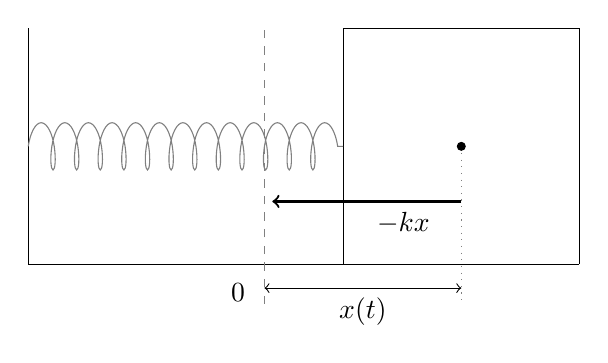
\begin{tikzpicture}
\draw[-] (0,0) -- (7,0);
\draw[-] (0,0) -- (0,3);

\draw[-] (4,0) -- (4,3) -- (7,3) -- (7,0);

\draw[gray,dashed] (3,-0.5) -- (3,3);
\draw[gray,dotted] (5.5,1.5) -- (5.5,-0.5);
\draw[thick,->] (5.5,0.8) -- node[below right, fill=white] {$-kx$} (3.1,0.8);
\node[label=below left:{$0$}] at (3,0) {};

\draw[gray,decoration={aspect=0.3, segment length=3mm, amplitude=3mm,coil},decorate] (0,1.5) -- (4,1.5);

\draw[<->] (3,-0.3) -- node[below] {$x(t)$} (5.5,-0.3);
\node[draw, fill=black, circle, inner sep=1pt] at (5.5,1.5) {};
\end{tikzpicture}
\caption{Sistema masa-resorte, con la fuerza del muelle $-kx$.}
\label{imgMasaResorte1}
\end{figure}

Según la ley de Hooke, la fuerza será

\[ F = -kx \]

donde $k$ es una constante que depende del muelle. Por la segunda ley de newton, tenemos que la fuerza es el producto de la masa y la aceleración, por tanto, la ecuación que describe el movimiento es

\[ mx'' = -kx \]

Podemos transformarla a un problema en derivadas ordinarias

$$\left\lbrace \begin{array}{l}
x'' + \frac{k}{m}x = 0\\
x(0) = x_0\\
x'(0) = v_0
\end{array}\right. $$

para el que necesitaremos posición y velocidad iniciales.

El polinomio característico es

\[ λ^2 + \frac{k}{m} = 0 \]

cuyas raíces son

\[ λ=\pm \imath \sqrt{\frac{k}{m}} \]

Las soluciones complejas son, por lo tanto,

\begin{gather*}
z_1 = e^{\imath t\sqrt{\frac{k}{m}}} = \cos \sqrt{\frac{k}{m}} t + \imath\sin \sqrt{\frac{k}{m}} t \\
z_1 = e^{-\imath t\sqrt{\frac{k}{m}}} = \cos \sqrt{\frac{k}{m}} t - \imath\sin \sqrt{\frac{k}{m}} t 
\end{gather*}

Combinándolas de forma lineal, obtenemos dos soluciones reales:

\begin{gather*}
x_1(t) = \Re (z_1) = \cos \sqrt{\frac{k}{m}} t \\
x_2(t) = \Im (z_1) = \sin \sqrt{\frac{k}{m}} t
\end{gather*}

Aunque se ve a simple vista que esas dos soluciones son independientes (el coseno y el seno del mismo ángulo), deberíamos calcular el Wronskiano para comprobar que son realmente independientes.

La solución general nos queda

\begin{equation}\label{eqMasaResorte} x(t) = A\cos \sqrt{\frac{k}{m}} t + B \sin \sqrt{\frac{k}{m}} 
\end{equation}

Las constantes $A$ y $B$ se tendrán que obtener una vez dados los valores iniciales. Si suponemos $x(0) = x_0$, $x'(0) = v_0$, tenemos que

\begin{align*}
x_0 &= x(0) = A \\
x'(t) &= -x_0 \sqrt{\frac{k}{m}} \sin \sqrt{\frac{k}{m}} t + B \sqrt{\frac{k}{m}}\cos\sqrt{\frac{k}{m}} t \\
v_0 &= x'(0) = B \sqrt{\frac{k}{m}} \\
B &= \frac{v_0}{\sqrt{\frac{k}{m}}}
\end{align*}

Si bien esta solución es correcta, los físicos suelen reescribirla de una forma distinta utilizando coordenadas polares para el punto $(A,B)$:

\begin{align*}
A &= R\cos φ \\
B &= R\sin φ
\end{align*}

Sustituyendo en \eqref{eqMasaResorte}

\[ x(t) = R\left(\cos \sqrt{\frac{k}{m}} t\cos φ + \sin \sqrt{\frac{k}{m}} t \sin φ \right) = R\cos\left(\sqrt{\frac{k}{m}}t - Φ\right) \]

donde $Φ = \arctan \frac{B}{A}$ es el desfase, que actúa de velocidad inicial del sistema.

\paragraph{Sistema masa-resorte con rozamiento}

Replanteemos el problema anterior con rozamiento.
\begin{figure}
\centering
\begin{tikzpicture}
\draw[-] (0,0) -- (7,0);
\draw[-] (0,0) -- (0,3);

\draw[-] (4,0) -- (4,3) -- (7,3) -- (7,0);

\draw[gray,dashed] (3,-0.5) -- (3,3);
\draw[gray,dotted] (5.5,1.5) -- (5.5,-0.5);
\draw[thick,->] (5.5,2) -- node[above right, fill=white] {$-εx'$} (2.7,2);
\draw[thick,->] (5.5,0.8) -- node[below right, fill=white] {$-kx$} (3.1,0.8);
\node[label=below left:{$0$}] at (3,0) {};

\draw[gray,decoration={aspect=0.3, segment length=3mm, amplitude=3mm,coil},decorate] (0,1.5) -- (4,1.5);

\draw[<->] (3,-0.3) -- node[below] {$x(t)$} (5.5,-0.3);
\node[draw, fill=black, circle, inner sep=1pt] at (5.5,1.5) {};
\end{tikzpicture}
\caption{Sistema masa-resorte con rozamiento (fuerza $-εx'$).}
\end{figure}

La ecuación cambia al añadir el rozamiento:

\begin{gather} mx'' = -kx - εx' \nonumber \\
x'' + \frac{ε}{m}x' + \frac{k}{m}x = 0
\end{gather}

Resolvemos el polinomio característico \[ λ^2 + \frac{ε}{m}λ + \frac{k}{m} = 0 \] y nos queda

\[ λ = \frac{-ε}{2m} \pm \sqrt{\left(\frac{ε}{2m}\right)^2 - \frac{k}{m}} \].

Tenemos que plantear tres casos basados en el valor de $Δ =\left(\frac{ε}{2m}\right)^2 - \frac{k}{m}$: si es mayor, igual o menor que cero.

\subparagraph{Primer caso: $Δ > 0$ (rozamiento alto)}

Tenemos

\begin{gather*}
λ_+ = \frac{-ε}{2m} + \sqrt{\left(\frac{ε}{2m}\right)^2 - \frac{k}{m}} \\
λ_- = \frac{-ε}{2m} - \sqrt{\left(\frac{ε}{2m}\right)^2 - \frac{k}{m}} 
\end{gather*}

De sus expresiones vemos que tanto $λ_+$ como $λ_-$ son negativos, puesto que la raíz siempre será menor que $\frac{\epsilon}{2m}$. La solución general del problema es

\[ x(t) = Ae^{λ_+t} + Be^{λ_-t} \]

Despejando de los valores iniciales $x(0) = x_0$, $x'(0) = v_0$ y realizando ciertas operaciones,

\[ x(t) = \frac{1}{λ_+ - λ_-}\left((v_0-λ_-x_0)e^{λ_+t} - (v_0-λ_+x_0)e^{λ_-t}\right) \]

De esa ecuación vemos que, cuando $t\to ∞$, $x(t) \to 0$. Es decir, el objeto tiende a pararse.

También querríamos ver cuántas veces pasamos por la posición de equilibrio. Tenemos que resolver la ecuación

\[ e^{(λ_+ - λ_-)t} = \frac{v_0-λ_+x_0}{v_0-λ_-x_0} \]

que no tiene solución (la exponencial es siempre positiva, pero la división es menor que 1). Por lo tanto, el objeto no llega nunca a la posición de equilibrio.

\subparagraph{Segundo caso: $Δ=0$}

En este caso, tenemos $λ=\frac{-ε}{2m}$ que es una raíz doble. Por el método de variación de las constantes, nuestras dos soluciones son

\[ x_1(t) = e^{\frac{-ε}{2m}t};\quad x_2(t) = te^{\frac{-ε}{2m}t} \]

y la solución general se expresa como

\[ x(t) = A e^{\frac{-ε}{2m}t} + B t e^{\frac{-ε}{2m}t} = e^{\frac{-ε}{2m}t} \left(A + Bt\right) \]

Al igual que en el anterior caso, $x(t) \convs[][t][∞] 0$, pero aquí sí que podemos tener soluciones para $x(t) = 0$. La existencia o no de una solución dependerá de la posición y velocidad iniciales.

\subparagraph{Tercer caso: $Δ < 0$ (sin rozamiento)}

Aquí tendremos raíces complejas, es decir:

\[ λ_+ = \frac{-ε}{2m} + \imath\sqrt{\frac{k}{m} - \left(\frac{ε}{2m}\right)^2} \]

y su conjugada. De esta forma, las dos soluciones reales serán

\begin{gather*}
x_1(t) = e^{\frac{-ε}{2m}t} \cos t\sqrt{\frac{k}{m} - \left(\frac{ε}{2m}\right)^2} \\
x_1(t) = e^{\frac{-ε}{2m}t} \sin t\sqrt{\frac{k}{m} - \left(\frac{ε}{2m}\right)^2} \\
\end{gather*}

Podemos extraer la solución general y hacer el cambio del anterior apartado, pasando a polares $(A,B) \sim (R\cos φ, R\sin φ)$, de tal forma que nos queda la solución general

\[ x(t) = R e^{-\frac{ε}{2m}t} \cos \left(t\sqrt{\frac{k}{m} - \left(\frac{ε}{2m}\right)^2} - φ\right) \]

Es decir, hay un decaimiento exponencial de la amplitud. La gráfica de la función sería la de la \textbf{Figura \ref{fig:imgMasaResorteSeno}}

\img{img/MasaResorteSeno.png}{$x(t)$ para un sistema masa-resorte}{imgMasaResorteSeno}{0.8}

\paragraph{Péndulo simple}

Consideramos un péndulo simple sin rozamiento.

\begin{figure}[hbtp]
\centering
\begin{tikzpicture}
\node (O) at (0,0) {};
\node (Vert) at (0,-2) {};
\node (P) at (1,-2) {};

\draw[-] (-2,0) -- (2,0);
\draw[-] (0,1) -- (O.center);
\draw[dashed] (O.center) -- (0,-4);

\draw[-] (O.center) -- (P.center);
\draw[->] (P.center) -- node[right] {$mg$} (1,-3.5);
\node[draw, fill=gray, circle, inner sep=4pt] at (P) {};

\tikzangle[name=$\theta$]{O.center}{P.center}{Vert.center}
\end{tikzpicture}
\caption{El péndulo}
\end{figure}

Tenemos las ecuaciones de posición

\[ σ(t) = (L\sin θ(t), - L \cos θ(t))\]

de velocidad

\[ σ'(t) = (Lθ'(t)\cos θ(t), Lθ'(t)\sin θ(t))\]

y aceleración

\begin{align*}
 σ''(t) = (&-L(θ'(t))^2\sin(t) + Lθ''(t)\cos(t), \\
 & L(θ'(t))^2\cos θ(t) + Lθ''(t)\sin θ(t)) 
 \end{align*}.

Por la segunda ley de Newton, tenemos que la fuerza ejercida es igual al producto de la masa y la aceleración. Si dividimos la cuerda en su componente tangencial y perpendicular tenemos:

\[ mg( -\cosθ, -\sin θ)\sin θ  = m σ''(t) \]

y por lo tanto nos quedan las dos ecuaciones
\[
\left\{\begin{matrix}
 -g\sin θ \cos^2 θ = -L θ'^2 \cos θ \sin θ+ Lθ''\cos^2θ  \\
 -g\sin θ \sin^2 θ = -L θ'^2 \sin θ \cos θ  + Lθ''\sin^2θ  
 \end{matrix}\right\} \]

 La ecuación final es \[ -g\sin θ = L θ'' \] o, transformada

 \[ θ'' + \frac{g}{L} \sin θ = 0 \]

Por Taylor, podemos aproximar $\sin θ \sim θ$ cuando θ es pequeña, de tal forma que nos reducimos al caso de un sistema masa-resorte.

\subsection{Problemas lineales no homogéneos con coeficientes constantes}

¿Qué ocurre cuando consideramos sistemas con fuerzas externas? Un ejemplo sería la siguiente ecuación en orden dos:

\begin{equation}
\label{eqEcOrden2} x'' + ax' + bx = f(t)
\end{equation}

en la que $f(t)$ representa esa fuerza externa. Tal y como habíamos visto en anteriores secciones, la solución general $X_G$ se escribía como una solución particular $X_P$ más todas las asociadas al homogéneo $X_H$. En esta situación el problema es encontrar la solución particular, para lo cual teníamos varios métodos.

\subsubsection{Método de variación de constantes}
\label{secMetodoVarConst}
\index{Variación!de constantes}

Siguiendo con el ejemplo en orden 2, tenemos

\[ x_H (t) = c_1x_1(t) + c_2x_2(t) \]
y buscamos una solución en la que
$$
\left\lbrace
\begin{array}{l}
c_1 = c_1(t)\\
c_2 = c_2(t)
\end{array}
\right.
$$
Por tanto buscamos $X_P$ tal que
\[ x_P(t) = c_1(t)x_1(t) + c_2(t)x_2(t) \] Para ello derivamos:
\begin{align*}
x_P'&= c_1'x_1 + c_1x_1' + c_2'x_2 + c_2x_2' \\
x_P'' 	&= c_1''x_1+c_1'x_1' + c_2''x_2+c_2'x_2' + \\
		&\quad+ c_1'x_1'+c_1x_1'' + c_2'x_2' + c_2x_2'' = \\
		&= c_1''x_1 + c_2''x_2+2c_1'x_1'+2c_2'x_2' + c_1x_1'' +c_2x_2''
\end{align*}

Sustituyendo en \eqref{eqEcOrden2}:

\begin{align*}
f(t) &= x_P'' + ax_P' + bx_P = &  \\
	&= c_1''x_1 + c_2''x_2 + 2c_1'x_1' + 2c_2'x_2'  + c_1x_1''  + c_2x_2'' \\
	& + ac_1' x_1 + ac_2'x_2  + ac_1x_1'  + ac_2x_2' \\
	&  + bc_1x_1  + bc_2x_2 
\end{align*}

Tras la sustitución tenemos una expresión bastante compleja. Sin embargo, recordamos que no buscamos todas las soluciones de la ecuación, sino que basta con encontrar sólo una. Por ello, planteamos ciertas condiciones para resolver la expresión hallada:

$$ \left\lbrace \begin{array}{l}
c_1'x_1 + c_2'x_2 = 0 \\
c_1'x_1' + c_2'x_2' = f
\end{array} \right. $$
Que nos lleva al sistema

\[ \underbrace{\begin{pmatrix}
x_1 & x_2 \\
x_1' & x_2'
\end{pmatrix}}_A\begin{pmatrix}
c_1' \\ c_2'
\end{pmatrix} = \begin{pmatrix}
0 \\ f(t)
\end{pmatrix} \]
Se puede observar que el sistema tiene solución, ya que al ser $x_1,\ x_2$ soluciones independientes, el Wronskiano (en este caso, el determinante de $A$) es distinto de $0$.

En un caso general de orden $n$, el sistema a plantear tendrá la siguiente forma

\[ \begin{pmatrix}
x_1 & \cdots & x_n \\
x_1' & \cdots & x_n \\
\vdots & \ddots & \vdots \\
x_1^{n-1)} & \cdots & x_n^{n-1)}
\end{pmatrix} \begin{pmatrix} c_1' \\ c_2' \\ \vdots \\ c_n' \end{pmatrix}
=
\begin{pmatrix}
0 \\ \vdots \\ 0 \\ f(t)
\end{pmatrix} \]
Veamos un ejemplo.

\begin{example}
$x'' + x = e^t$

Buscamos $x_P(t) = c_1(t) x_1 + c_2(t) x_2$, donde

\[ \underbrace{\begin{pmatrix}
x_1 & x_2 \\
x_1' & x_2'
\end{pmatrix}}_A\begin{pmatrix}
c_1' \\ c_2'
\end{pmatrix} = \begin{pmatrix}
0 \\ e^t
\end{pmatrix} \]

Podemos elegir $x_1$ y $x_2$ como el seno y el coseno de $t$:

\[ \underbrace{\begin{pmatrix}
\cos t & \sin t \\
- \sin t & \cos t
\end{pmatrix}}_A\begin{pmatrix}
c_1' \\ c_2'
\end{pmatrix} = \begin{pmatrix}
0 \\ e^t
\end{pmatrix} \]
Resolviendo el sistema nos queda que

\[ c_2' = e^t \cos t \]

Realizando bastantes operaciones podemos obtener una solución particular, sin embargo, podemos darnos cuenta de que una de las soluciones particulares es

\[ x_p(t) = \frac{e^t}{2} \]

¿Qué tiene de especial este problema? La exponencial en $f(t)$. Lo que nos lleva a estudiar otro método, el de coeficientes indeterminados.
\end{example}


\subsubsection{Método de coeficientes indeterminados}

Podremos aplicar este método cuando $f(t)$ sea un polinomio, una exponencial, senos y cosenos y combinaciones lineales de todos los anteriores. En todos estos casos las derivadas nos llevan a funciones de la misma clase, y podremos aplicar este método que nos lleva a cuentas más sencillas.

En este método, suponemos que la solución particular es una función de la misma familia de $f(t)$ multiplicada por una constante, así que planteamos el problema y resolvemos el sistema. Estudiémoslo desde un ejemplo:

\paragraph{1) Exponenciales} \[ x'' - x = e^{2t} \]

Tenemos que
\begin{gather*}
x_p(t) = Ce^{2t} \\
x_p' = 2Ce^{2t} \\
x_p'' = 4Ce^{2t} \\
e^2t = 4Ce^{2t} - Ce^{2t} = 3Ce^{2t}
\end{gather*}

$C$ ha de ser $\frac{1}{3}$ y por lo tanto nuestra solución general del sistema será

\[ x_G = c_1e^t + c_2e^{-t} + \frac{1}{3}e^{2t} \]

\paragraph{2) Exponenciales con $f(t)$ solución de la homogénea} Otro ejemplo:

\[ x''-x= e^t \]

Aquí habría que calcular $x_p = ce^t$. Sin embargo, tomando esa solución nos quedaría $x_p'' - x_p = 0\; ∀c$, por lo que no nos vale. Cuando $f(t)$ es una de las soluciones de la ecuación homogénea asociada, tenemos que añadir algo más. Buscamos soluciones de la forma $cte^t$

\begin{gather*}
x_p  = cte^t \\
x_p' = cte^t + ce^t \\
x_p'' = cte^t + 2ce^t \\
\end{gather*}

Resolviendo:

\begin{align*}
x_p'' - c_p &= 2ce^t \\
e^t &= 2ce^t \\
C &= \frac{1}{2}
\end{align*}

\paragraph{3) Senos y cosenos} Probamos ahora con senos y cosenos.

\[ x'' + x= \cos 2t\]

En este caso, la solución debe tener una combinación lineal de senos y cosenos. Por lo tanto

\[ x_p = A\cos 2t + B\sin 2t \]

y resolviendo

\[ \cos 2t = x_p'' + x_p = -3A\cos 2t - 3B\sin 2t \]

de tal forma que $A=\frac{-1}{3}$ y $B=0$.

\paragraph{4) Senos y cosenos con $f(t)$ sol. de la homogénea} Consideramos $x''+x = \cos t$.

En este caso, $f(t) = \cos t$ es una solución de la parte homogénea, así que la solución será de la forma

\[ x_p(t) = At\cos t + Bt\sin t \]

Supongamos que esto modela una situación real, como por ejemplo empujando un columpio. ¿Cómo interpretamos esto?

A ciertas frecuencias, la ecuación es creciente, la amplitud aumenta con el tiempo. Es un fenómeno de \textbf{resonancia}. Veamos cómo modelizar este caso.

\paragraph{Ejemplo: Sistema masa-resorte con fuerza externa (sin rozamiento)}

La ecuación en este caso es

\(\label{eqMRF1} x'' + \underbrace{\frac{k}{m}}_{=ω^2}x = \underbrace{f(t)}_{F\cos αt} \)

Hemos cambiado algunas constantes para adaptarlo a nuestro caso. Hay varias opciones a partir de aquí relacionadas con las constantes ω y α:

\subparagraph{Caso 1: $ω≠α$}

Resolvemos la ecuación homogénea $x''+ω^2 x = 0$ con el polinomio característico:

\[ λ^2+ω^2  = 0 \implies λ = \pm ω\imath \]

y por lo tanto

\( x_H(t) = c_1 \cos ωt + c_2 \sin ωt \)

Necesitamos ahora una solución particular $x_P = A\cos αt + B\sin αt$. Derivamos dos veces:

\begin{align*}
x_P(t) &= A\cos αt + B\sin αt \\
x_P'(t) &= -Aα\sin αt + Bα\cos αt \\
x_P''(t) &= -Aα^2\cos αt - Bα^2\sin αt 
\end{align*}

Sustituyendo en \eqref{eqMRF1}

\begin{gather*}
 F\cos αt = x_P'' + ω^2x_P = \dotsb = (ω^2-α^2)\left(A\cos αt + B\sin αt\right) \\
 B = 0;\quad A= \frac{F}{ω^2-α^2} \\
 x_P(t) = \frac{F}{ω^2-α^2}\cos αt
\end{gather*}

De esta forma, la ecuación general nos queda

\( x_G(t) = \frac{F}{ω^2-α^2}\cos αt + c_1 \cos ωt + c_2 \sin ωt \)

Para los datos iniciales $x(0) = x'(0) = 0$, despejamos y tenemos la solución al problema

\(\label{eqMRF2-Sol} x(t) = \frac{F}{ω^2-α^2}\left(\cos αt - \cos ωt\right) \)

Volviendo de nuevo al sistema que tratamos, ω y α representan dos frecuencias. α es la externa y ω es la natural. Podemos reescribir la ecuación \eqref{eqMRF2-Sol} usando identidades trigonométricas. Sabemos que

\[ \cos (A-B) - \cos(A+B) = 2\sin A \sin B \]

Resolvemos:

\[ \left.\begin{matrix}A - B = αt \\ A + B = ωt \end{matrix}\right\}
\left.\begin{matrix}A = \frac{ω+α}{2}t \\ B = \frac{ω-α}{2}t\end{matrix}\right\} \]

Sustituyendo en \eqref{eqMRF2-Sol}:

\( x(t) = \frac{2F}{ω^2-α^2} ·\sin\left( \frac{ω-α}{2}t\right) · \sin\left( \frac{ω+α}{2}t\right)  \)

Luego lo que tenemos es una oscilación rápida (Δ) con una amplitud contenida dentro de otra con oscilación más lenta (Γ).

\begin{figure}
\centering
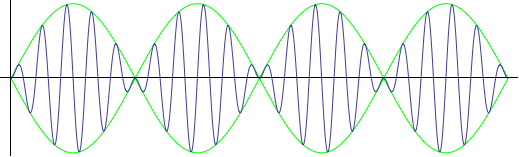
\includegraphics[width=0.8\textwidth]{img/MasaResorteF.png}
\caption{Gráfico de una oscilación rápida (Δ, azul) con una amplitud contenida dentro de otra con oscilación más lenta (Γ, verde)}
\label{imgMasaResorteF}
\end{figure}

\subparagraph{Caso 2: $ω=α$}

En este caso, la ecuación diferencial es

\[ x'' + ω^2 x = F\cos ωt \]

La solución de la homogénea es $x_H = c_1 \cos ωt + c_2 \sin ωt$. Tenemos un problema: $F\cos ωt$ es solución de la homogénea. Para encontrar una solución particular multiplicamos entonces por $t$:

\begin{gather*}
x_P = t\left(A\cos ωt + B\sin ωt\right) \\
x_P' =t\left(-Aω\sin ωt + Bω\cos ωt\right) + \left(A\cos ωt + B\sin ωt\right) \\
x_P'' = t\left(-Aω^2 \cos ωt - Bω^2 \sin ωt\right) + 2\left(-Aω\sin ωt + Bω\cos ωt \right)
\end{gather*}

Igualando,

\[ F\cos ωt \stackrel{?}{=} x_p'' + ω^2x_p = 2\left(-Aω\sin ωt + Bω\cos ωt \right) \]

de donde sacamos que $A=0$ y $B=\frac{F}{2ω}$. Una solución particular es entonces

\[ x_P(t) = \frac{F}{2ω}t \sin ωt \]

que es además la solución que cumple $x_P(0) = x_P'(0) = 0$. La gráfica de esta ecuación será

\begin{figure}[hbtp]
\centering
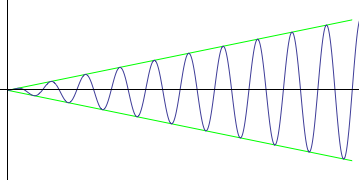
\includegraphics[width=0.5\textwidth]{img/MasaResorteF-Resonancia.png}
\caption{Gráfica de un sistema masa-resorte en resonancia}
\label{imgMasaResorteFR}
\end{figure}

Estamos ante un fenómeno de resonancia. La amplitud tiene a infinito siempre, por muy pequeña que sea la fuerza.

Que, por cierto, Azorero nos ha engañado en una cosa: la expresión de la fuerza es un coseno en lugar de una función genérica $F(t)$. En realidad esto se debe al desarrollo en serie de Fourier, que dice que cualquier función se puede expresar como

\[ F(t) = \sum_{j=0}^∞ F_j \cos \frac{jπ}{T}t \]

\paragraph{Modelo con rozamiento}

Añadiendo el rozamiento al modelo anterior, tenemos

\[ x''+2εx'+ω^2x = \cos αt \]

Haciendo cuentas y suponiendo $ε^2-ω^2<0$. Nos queda una solución para la homogénea

\[ x_H = e^{-εt}\left(c_1 \cos \left( \sqrt{ω^2-ε^2}t \right) + c_2 \sin \left( \sqrt{ω^2-ε^2}t\right)\right) \]

Buscamos la solución particular

\[ x_P (t) = A\cos αt + B\sin αt \]

y llegamos a

\[ x_P(t) = \frac{1}{(ω^2-α^2)^2 + 4α^2ε^2}\left((ω^2-α^2)\cos αt + 2αε \sin αt \right) \].

La solución general es entonces

\[ x_G(t) = x_P(t) + x_H(t) \]

Dado que en $x_H$ está todo multiplicado por una exponencial negativa, tiende a cero cuando $t\to ∞$, por lo que la llamamos la parte \textbf{transitoria}. El primer sumando, $x_P$, permanece y se le llama la parte \textbf{estacionaria}.

En este caso, cuando $α=ω$ (estamos en la frecuencia de resonancia), es el que más aporta a la ecuación. Sin embargo, en ningún caso la amplitud se va a infinito. El rozamiento impide que la amplitud se dispare.

\subsubsection{Resumen de métodos para ec. lineales no homogéneas}

Hagamos un resumen de los métodos que hemos visto. Las soluciones de una ecuación no homogénea de la forma

\[ y^{n)} + a_{n-1}y^{n-1)} + \dotsb + a_1y'+a_0y = f(t) \]

se expresan en función de una solución particular $y_p$ y el conjunto de las soluciones para la ecuación homogénea asociada $y_H$:

\[ y_G = y_p + y_H \]

Podemos obtener fácilmente las soluciones a la homogénea usando la técnica vista en la sección anterior \eqref{secEcHomoLinealConstante}. Para obtener la solución particular tenemos que usar el método de variación de constantes (\ref{secMetodoVarConst}). Sin embargo, ese método nos lleva a muchas más cuentas de las necesarias. Podemos simplificar las cosas cuando $f(t)$ pertenece a una familia de curvas "cerrada" por la derivada. Veamos esos casos.

\paragraph{Polinomio}

\[ f(t) = A_0 + A_1t + \dotsb + A_Nt^N \]

Si $0$ no es raíz, buscamos \[y_p(t) = a_0 + a_1t + \dotsb + a_Nt^N\]. Si $0$ es raíz con multiplicidad $k$, entonces la solución particular que buscamos será de la forma

\[ y_p(t) =( a_0 + a_1t + \dotsb + a_Nt^N)t^k \]

\paragraph{Trigonométrico}

\[ f(t) = \cos αt \]

o análogamente para senos. Tenemos dos posibilidades. Si $α\i$ no es raíz del p. característico, la solución particular es de la forma

\[ y_p(t) = a\cos αt + b\sin αt \]

En el caso de que $α\imath$ sea raíz con multiplicidad $k$, entonces

\[ y_p(t) = (a\cos αt + b\sin αt)t^k \]

\paragraph{Polinomio y exponencial}

\[ f(t) = e^{αt}(A_0 + A_1t + \dotsb + A_Nt^N) \]

Si $α$ no es raíz del p. característico,

\[ y_p(t) = e^{αt}(a_0 + a_1t + \dotsb + a_Nt^N) \]. si α sí es raíz con multiplicidad $k$,

\[ y_p(t) = t^ke^{αt}(a_0 + a_1t + \dotsb + a_Nt^N) \]

\subsection{Ejemplos}

\begin{example} Consideramos la ecuación

\[ y'' + a' + by = 0 \]

Demuestra que

\[ y_H(t) \convs[][t][∞] 0 \iff a>0, b>0 \]

Empezamos por la implicación a la izquierda. El polinomio característico es

\[ λ^2+aλ+b \implies λ_{\pm} = \pm \frac{a\pm \sqrt{a^2-4b}}{2} \]

Tenemos tres casos:

\begin{itemize}
\item $a^2-4b > 0$. En este caso, $λ_-,λ_+ ∈ℝ$, $λ_-<λ_+<0$ y por lo tanto $e^{λ_+t}$ y $e^{λ_-t}$ tienden a cero cuando $t\to ∞$.

\item $a^2=4b$. Aquí tenemos que $λ=\frac{-a}{2}$, raíz doble. Las soluciones son $e^{\frac{-a}{2}t}$ y $te^{\frac{-a}{2}t}$, ambas tienden a cero.

\item $a^2-4b > 0$. Las raíces son imaginarias y te sale igual porque lo ha borrado.

\end{itemize}

Para demostrar la implicación a la derecha, tenemos que si $y_H(t)\convs[][t][∞]0$, entonces los autovalores del p.c. son o bien

\[ y_\pm = α\pm + \iβ \]

con $α<0$ o bien reales con $λ_-≤λ_+<0$. En ambos casos tenemos que $a>0, b>0$ tal y como hemos visto al demostrar la otra implicación.

\end{example}

\begin{example}[Ejercicio 7]

Tenemos la siguiente ecuación:

\[ y^{iv)} + 4y''' + 8y'' + 8y' +4y = 0\]

y nos dicen que $\imath- 1$ es raíz del p.c.

\[ P(λ) = λ^4 + 4λ^3 + 8λ^2 + 8λ + 4 = 0 \]

Sabiendo que $\i-1$ es raíz y que su conjugado $-\imath- 1$ también, podemos hacer las cuentas y

\begin{gather*}
 P(λ) = (λ-(-1+\i)) · (λ-(-1-\i)) · P_2(λ) \\
 ((λ+1)^2 + 1) P_2(λ)
 \end{gather*}

donde

\[ P_2(λ) = \frac{λ^4+ 4λ^3 + 8λ^2 + 8λ + 4 }{λ^2+2λ + 2} = \dotsb = λ^2 + 2λ + 2 \].

Por lo tanto las dos raíces son dobles.
\end{example}

\begin{example}[Ejercicio 8] Tenemos la ecuación

\[ y^{n)} + a_{n-1}y^{n-1)} + \dotsb + a_1y' + a_0y = x^k \]

con $a_0≠0$. Demostrar que en el caso $n=4,k=3$, existe un único polinomio que sea solución del problema, que además tiene grado 3.

Hay que demostrar dos cosas: que existe y que es único. Empezamos demostrando la unicidad suponiendo que existen $P,Q$ polinomios de grado tres solución.

En este caso tendríamos que $P-Q$ es solución de la homogénea. Y ha dicho algo y no lo he podido copiar.

Demostramos ahora la existencia. Buscamos una solución polinómica $y(x) = c_0+c_1x + c_2x^2 + c_3x^3$. Si calculamos

\[ a_0y(x) + a_1y'(x) + a_2y''(x) + a_3y'''(x) = x^3 = \underbrace{\{c_j,a_j\}}_{=0} + \underbrace{\{c_j,a_j\}x}_{=0} + \underbrace{\{c_j,a_j\}x^2}_{=0} + \underbrace{\{c_j,a_j\}}_{=1}x^3 \]

donde $\{c_j,a_j\}$ son combinaciones lineales de cada una de las $a_j$ y $c_j$. Tendremos entonces un sistema con coeficientes $a_j$ e incógnitas $c_j$ de la forma

\[ A \begin{pmatrix}
c_0 \\ c_1 \\ c_2 \\ c_3
\end{pmatrix} = \begin{pmatrix}
0 \\ 0 \\ 0 \\ 1
\end{pmatrix} \]
\end{example}

\begin{example}[Ejercicio 11 - Hoja 3]

Tenemos la ecuación

\[ y'' + P(t) y' + Q(t) y = 0 \]

Decir sobre qué condiciones de $P,Q$ el cambio de variables $s=Φ(t), z(s) = y(t)$ convierte la ecuación en una coeficientes constantes.

Calculamos las derivadas:

\begin{gather*}
 \od{y}{t} = \od{y}{t} \od{s}{t} = \od{z}{s} \od{Φ}{t} \\
 \od[2]{y}{t} = \od[2]{z}{s} \left(\od{Φ}{t}\right)^2 + \od{z}{s}\od[2]{Φ}{t}
\end{gather*}

y sustituyendo

\[ 0 = \od[2]{z}{s} + \underbrace{\left(\frac{\od[2]{Φ}{t} + P\od{Φ}{t}}{\left(\od{Φ}{t}\right)^2}\right)}_{A} \od{z}{s} + \underbrace{\frac{Q}{\left(\od{Φ}{t}\right)^2}}_{B}z \]

tenemos que buscar las condiciones sobre $P$ y $Q$ y la expresión de $Φ(t)$ para que ahí haya constantes multiplicando a $\od{z}{s}$ y a $z$. Entonces

\[ \frac{Q}{\left(\od{Φ}{t}\right)^2} = B \implies \left(\od{Φ}{t}\right)^2 = \frac{Q}{B} \implies \od{Φ}{t} = \sqrt{\frac{Q}{B}} \]

Sustituyendo:

\[ A = \frac{\od[2]{Φ}{t} + P\sqrt{\frac{Q}{B}}}{\left(\od{Φ}{t}\right)^2} \]

Casi tenemos la relación, pero tenemos que deshacernos de esa segunda derivada. Así que derivamos Φ:

\[ \od[2]{Φ}{t} = \frac{A}{2\sqrt{B}\sqrt{Q}}Q' \]

y sustituimos

\[ A = \frac{\frac{1}{2\sqrt{B}\sqrt{Q}}Q' + P\sqrt{\frac{Q}{B}}}{\left(\od{Φ}{t}\right)^2} = \dotsb = \frac{Q'+2PQ}{Q\sqrt{Q}} = \text{cte.} \]

y además tiene que ser

\[ (Φ'(t))^2 = \frac{Q(t)}{B} \]

\end{example}

